\begin{figure*}[!t]
\centering\small
\centering
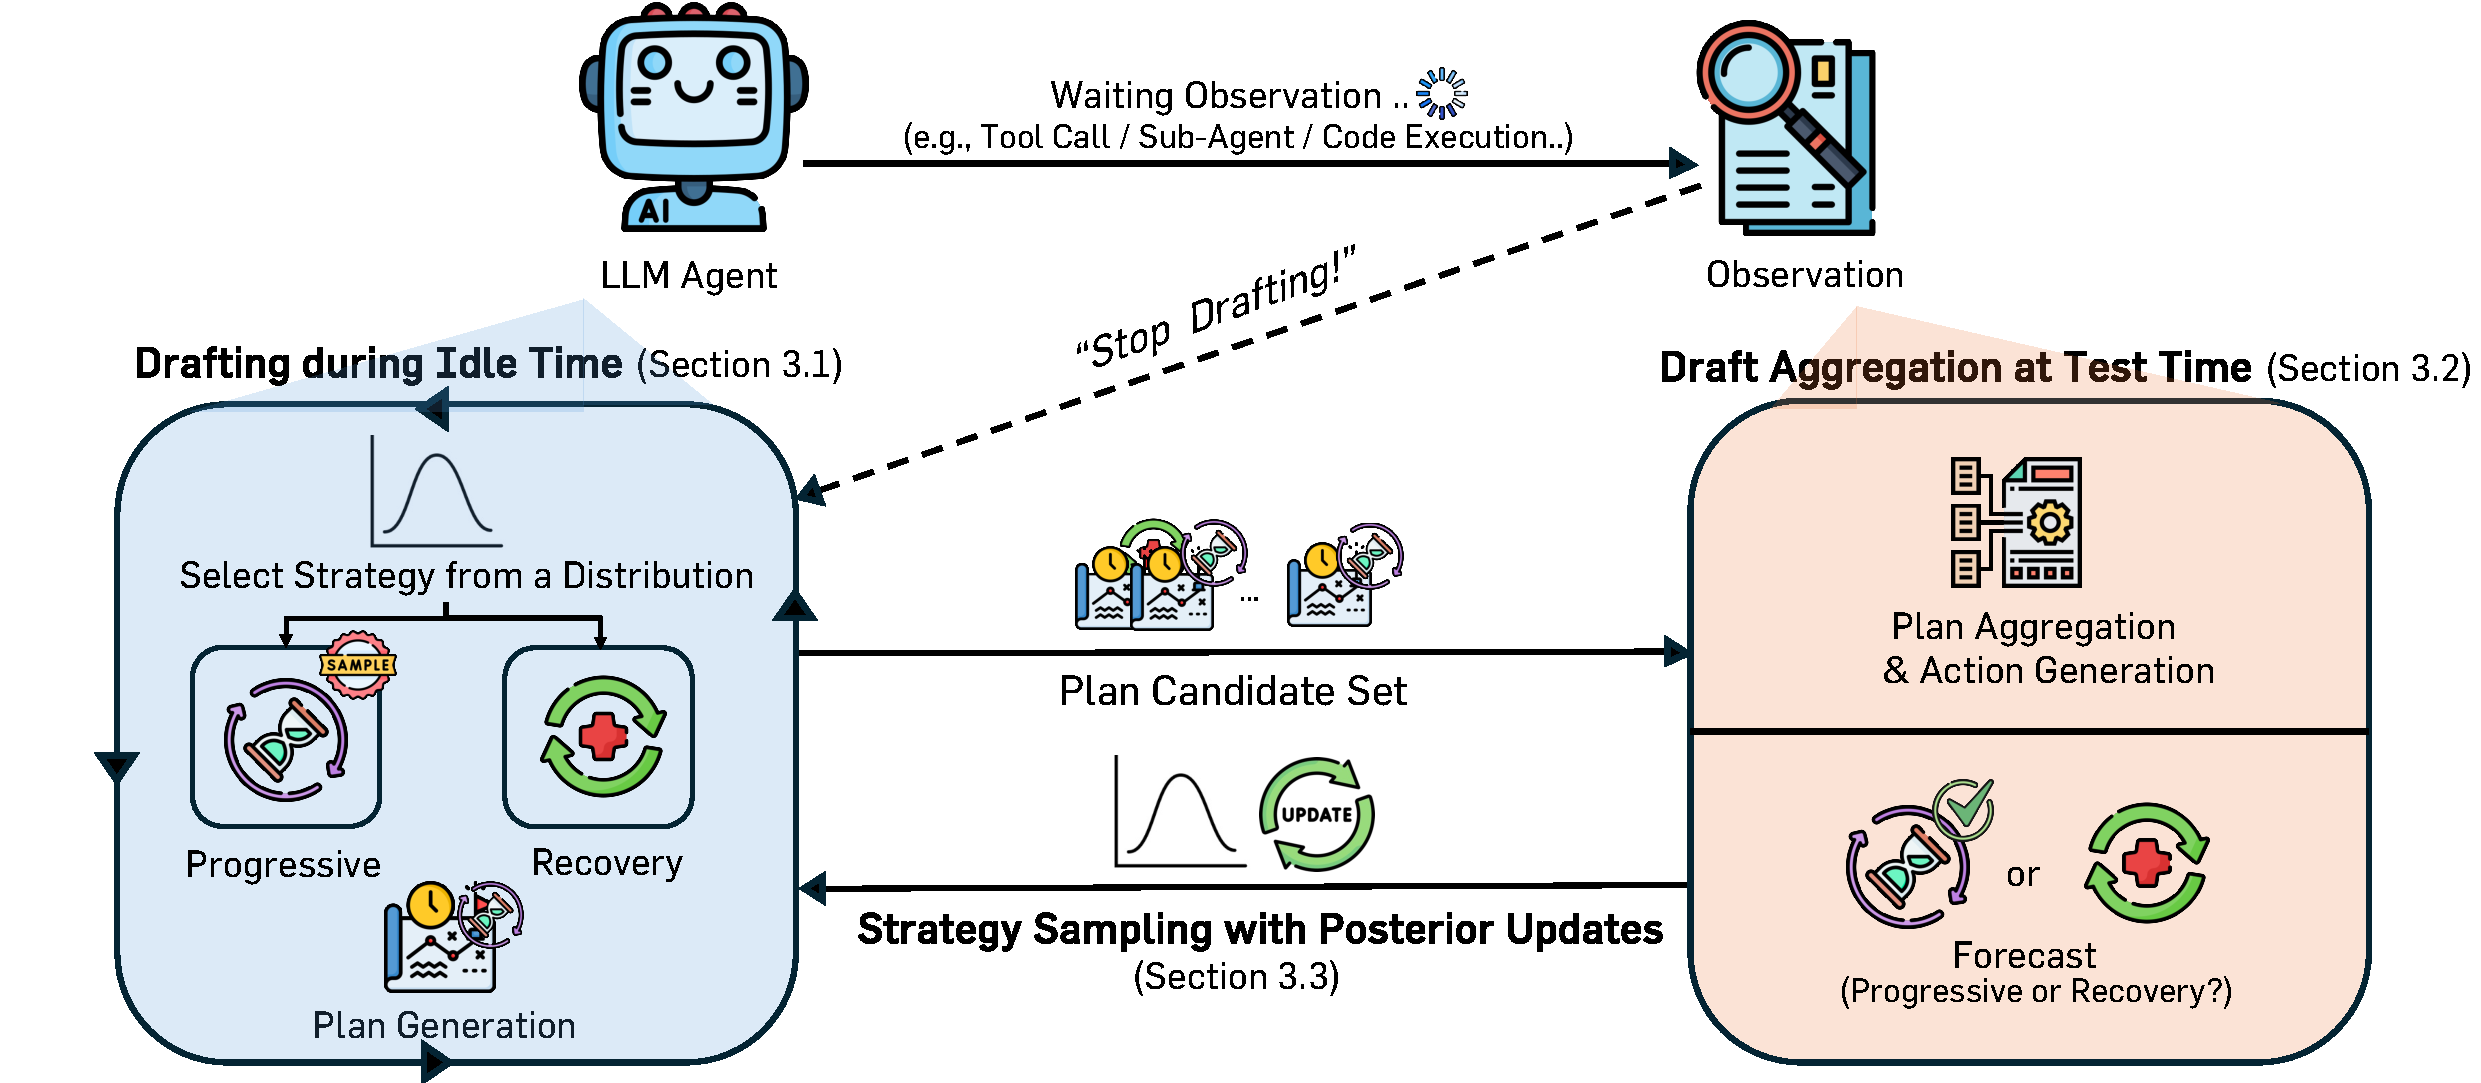
\includegraphics[width=\linewidth,height=0.45\linewidth]{figures/concept_figure.pdf}
\vspace{-2mm}
\caption{
\textbf{Overview of \mname.}
\textbf{(a) Idle-Time Drafting:} during tool execution, the agent iteratively drafts plan candidates by sampling between \textit{Progressive} and \textit{Recovery} strategies, and terminates drafting once the observation arrives.
\textbf{(b) Draft Aggregation:} the agent aggregates the candidates with the observation into a refined action and forecasts whether the trajectory is on track or requires recovery.
\textbf{(c) Posterior Update:} the forecast signal updates the strategy distribution, biasing future drafts toward strategies effective in the current context.
}
\label{fig:concept}
\vspace{-1em}
\end{figure*}